\begin{document}
\section*{凯恩斯交叉和乘数效应}

凯恩斯交叉%
  \footnote{教材称它为``收入—支出模型''}
是我们这门课的第一个模型, 它决定了短期内的均衡国民收入, 
同时也是下一章 IS-LM 模型的基础.

% 模型的主要特点包括: 
% \begin{itemize}
% \item 
%   ``需求侧''分析: 假设经济体\textbf{供给充裕}, 因此总产出由需求侧决定.
% \item 
%   假设经济体在 \underline{短期内}\textbf{供给充裕}, 因此总产出由需求侧决定.
% \end{itemize}
%\textit{注:}教材对凯恩斯交叉的描述存在错误, 具体我会在后文指出\footnote{我在阅读第二版教材时, 感觉其中错误比第一版又多了一些, 至少第十章如此. 鉴于此, 请同学们带着批判的眼光阅读教材. 之后再遇到错误较多以致影响理解时, 我会上传相关讲义, 请大家留意. }. 
%请同学们注意. 

\paragraph{计划支出}
类比计算 GDP 的支出法, 我们将计划支出分解为四个部分: 
\begin{equation}
E = C + \bar{I} + G + NX 
\label{eq:planned}  
\end{equation}
\begin{itemize}
\item
  这里等号左边的 $E$ 表示``计划支出''. 后面定义消费函数时, 我们还会用到``实际支出'', 它表示为字母 $Y$. 
\item
  由衡量 GDP 的会计恒等式可知, $Y$ 既是总支出, 也是总收入, 也是总产出.
\item
  方程~\eqref{eq:planned}中的 $\bar{I}$ 表示计划投资, 教材也把它称为固定投资. 
\end{itemize}

除了计划投资, 实际投资支出 $I$ 还包括``非计划投资'': $I = \bar{I} + I_{\text{非计划}}$.
教材也把 $I_{\text{非计划}}$ 称为存货投资. 


\paragraph{消费函数} $C = \alpha + \beta  Y$. 总消费($C$)是总收入($Y$)的函数.  

\begin{itemize}
\item 严格来说, 消费应为\textbf{可支配收入}的函数. 若考虑政府税收, 则消费函数应写作
$$
C = \alpha + \beta  (Y-T),  \text{ 其中 $T$ 表示税收. }
$$
\item 
  消费函数由凯恩斯在《通论》一书里提出, 函数中的 $\beta$ 被称为``边际消费倾向'' (MPC, \textit{Marginal Propensity to Consume}).
  \begin{quote}
    {\it ``无论我们是从现已了解的人类本性上看, 还是从经验中的具体事实来看, 我们可以具有很大的信心来使用一条基本心理规律. 这条规律就是:在一般情况下, 平均说来, 当人们收入增加时, 他们的消费也会增加, 但消费的增加不会像收入增加的那样多. '' ——《就业、利息与货币通论》}
  \end{quote}
  
\item
  理解消费函数: 从整个经济体的角度来看, \textbf{总消费}会随着\textbf{总收入}的上升而上升, 但消费的增加不会像收入增加的那样多.
  \begin{itemize}
  \item
    人活着就要消费. 随着社会总产出 (总收入)的上升, 总消费也会上升. 
  \item
    $ 0 < \beta < 1$. 见教材图10-4, P39.
  \end{itemize}
\end{itemize}

\begin{framed}
\textbf{注1:} \textit{有同学问教材图 10-4 中的 $45^\circ$线有什么涵义, 这是个好问题. 书上的这个图画得不好, 应该用虚线来表示这个$45^\circ$线, 因为它没有啥实际涵义, 仅仅是用来和消费函数的线进行比较的. 
大家可以发现它没有消费函数陡峭, 所以 $\beta < 1$.}  
\end{framed}


\paragraph{均衡收入(均衡产出, 均衡支出)}
将消费函数代入表示支出法的方程  (1),  可得
\[ E = \alpha + \beta Y + \bar{I} + G + NX\]
均衡条件:实际支出 = 计划支出. 即 $Y=E$. 可得到如下决定均衡收入 $Y^*$
的方程:
\[Y^* = \alpha + \beta Y^* + {I} + G + NX \tag{2}\]
因为均衡时没有非计划投资, 所以我在方程(2)中用实际投资 $I$ 替换了计划投资 $\bar{I}$. 只有在经济体处于均衡状态下, 才可以作这个替换 (即 $I = \bar{I}$).

对方程(2)进行代数运算, 可解出:
\[Y^* = \frac{1}{1-\beta}  (\alpha + {I} + G + NX) \tag{3}\]
我们将括号内的 $\alpha + I + G + NX$
称为``自发性支出'', 即家庭、企业和政府自主选择的支出水平. 

凯恩斯交叉的图示见图 \ref{fig:cross}. 和之前的\textbf{注1}不同,
图 \ref{fig:cross} 中的 $45^\circ$ 线是有实际涵义的,%
   \footnote{细心的同学会发现, 教材 P35 的交叉图里, 计划支出写的是 E = C + I 而非 C + $\bar{I}$. 这里教材是错的;不仅如此, 教材里对计划支出 $E$ 的阐述也有许多小错. 编者要么并没有理解凯恩斯交叉模型, 要么是故意留下这些错误, 以待认真的同学发现$\,$:)}
它代表均衡条件, 即 $E=Y$.

\begin{figure}[H]
\centering
\begin{tikzpicture}
\tikzstyle{every node}=[font=\footnotesize] 
\coordinate  (A) at  (4, 0);
\coordinate  (B) at  (0, 4);
\coordinate  (eq) at  (2, 2);


\draw [<->]  (0, 5) --  (0, 0) --  (5, 0); % 坐标轴
\node [below] at  (4.5, 0) {$Y$ (实际支出)};
\node [left] at  (0, 5) {$E$};
\node [left] at  (0, 4.5) { (计划支出)};


\draw  (0, 0) --  (4, 4); % 均衡线
\draw  (0, 1) --  (2, 2) --  (4, 3); % 计划支出线
\node [below right] at  (4, 3) {$E = C + \bar{I} + G + NX$};
\node [right] at  (4, 4) {$Y = E$};

\draw[dashed]  (2, 0) --  (eq) --  (0, 2);
\node [below right] at  (eq) { \footnotesize 均衡};
\draw [fill]  (eq) circle [radius=0.03];

\draw  (0.2, 0.2) to [out =-45 , in=90]  (0.3, 0) ;
\node [above right] at  (0.3, 0) { \footnotesize $45^\circ$};

\end{tikzpicture}
\caption{凯恩斯交叉}
\label{fig:cross}
\end{figure}

\paragraph{乘数效应}   由于 $\beta \in  (0, 1)$,  所以公式  (3) 中系数 $\frac{1}{1-\beta} > 1$.
\begin{itemize}
  \item
    推论:自发性消费 $\alpha$,  自发性投资 $I$,  政府购买 $G$ 或净出口 \textit{NX}
    中任意一项增加一个单位, 经济产出都会扩张 $1/ (1-\beta)$ 倍, 这个倍数大于1. 
  \item
    这就是凯恩斯理论中的乘数效应  (multiplier effect):
    自发性支出的扩张会成倍地增加总产出. 这个倍数 $1/ (1-\beta)$
    被称为(自发性)支出乘数.

  \item
    \textit{乘数效应背后的经济学逻辑 (级数解释):} 大萧条时期, 若张三早上愿意多吃一碗 3
    元的米粉, 则社会的``自发性支出''增加 3 元, GDP
    增加了3元. 同时, 米粉店老板李四收入多了 3
    元, 根据线性消费函数的假设, 她的消费会增加 $3\beta$, 
    如找王五买了价值 $3 \beta$ 的奶茶. 同时, 王五的收入又多了
    $3 \beta$, 他会找赵六买$3 \beta^2$的饮料 ...
    这些新增的消费是一个无穷序列, 把它们加总后得到 $3 + 3 \beta + 3 \beta^2 + ... = 3/ (1-\beta)$.
    这个结果等于 3 乘上 multiplier.
  \end{itemize}

\subsection*{小结} 

凯恩斯交叉模型可表示为:
\begin{equation*}
\, \begin{cases}
E = C + \bar{I} + G + NX  &\text{(K1)} \\
C = \alpha + \beta Y &\text{(K2)}  \\
E =Y  &\text{(K3)}
\end{cases}  
\end{equation*}
其中方程 (K1) 表示计划支出, 可类比 GDP 计算的支出法进行理解;
方程 (K2) 表示消费函数, 参数 $\beta \in (0,1)$ 被称为边际消费倾向;
方程 (K3) 表示均衡条件, 计划支出等于实际支出 (或非计划支出等于0).

\begin{itemize}
\item 
  内生变量: $E$, $Y$, $C$.
\item 
  外生变量: 计划投资 $\bar{I}$, 政府购买 $G$, 净出口 $NX$, 自发性支出 $\alpha$, 边际消费倾向 $\beta$.  
\end{itemize}

\begin{framed}
\paragraph{练习} 考虑三部门经济  (即 NX = 0).
假设消费函数为 $C = 100 + 0.9 Y_d$, 其中 $Y_d$ 表示除去税收后的可支配收入, $I=300,  G=160,  T=0.2Y$. 计算  (1) 均衡国民收入水平  (2) 政府购买支出乘数  (3) 若 $G$ 增加到 300, 新的均衡收入是多少?  \hfill  (教材 P74Q4)
\end{framed}



\clearpage

\paragraph{乘数效应的应用: 用``凯恩斯交叉模型''来分析财政政策}

\begin{enumerate}
\def\labelenumi{\arabic{enumi}.}
\item
  政府购买乘数:政府增加1单位开支, 会通过乘数效应带来大于1单位的经济总产出的扩张. 因此, 政府应该在经济衰退时, 用扩张性的财政政策来管理总需求(即增大 G). 
  
  图 2: $G$ 上升 $\Rightarrow$ 计划支出线上移 $\Rightarrow$ 总产出扩张 $1/ (1-\beta)$ 倍

\begin{figure}[H]
\centering
\begin{minipage}{.55\textwidth}
  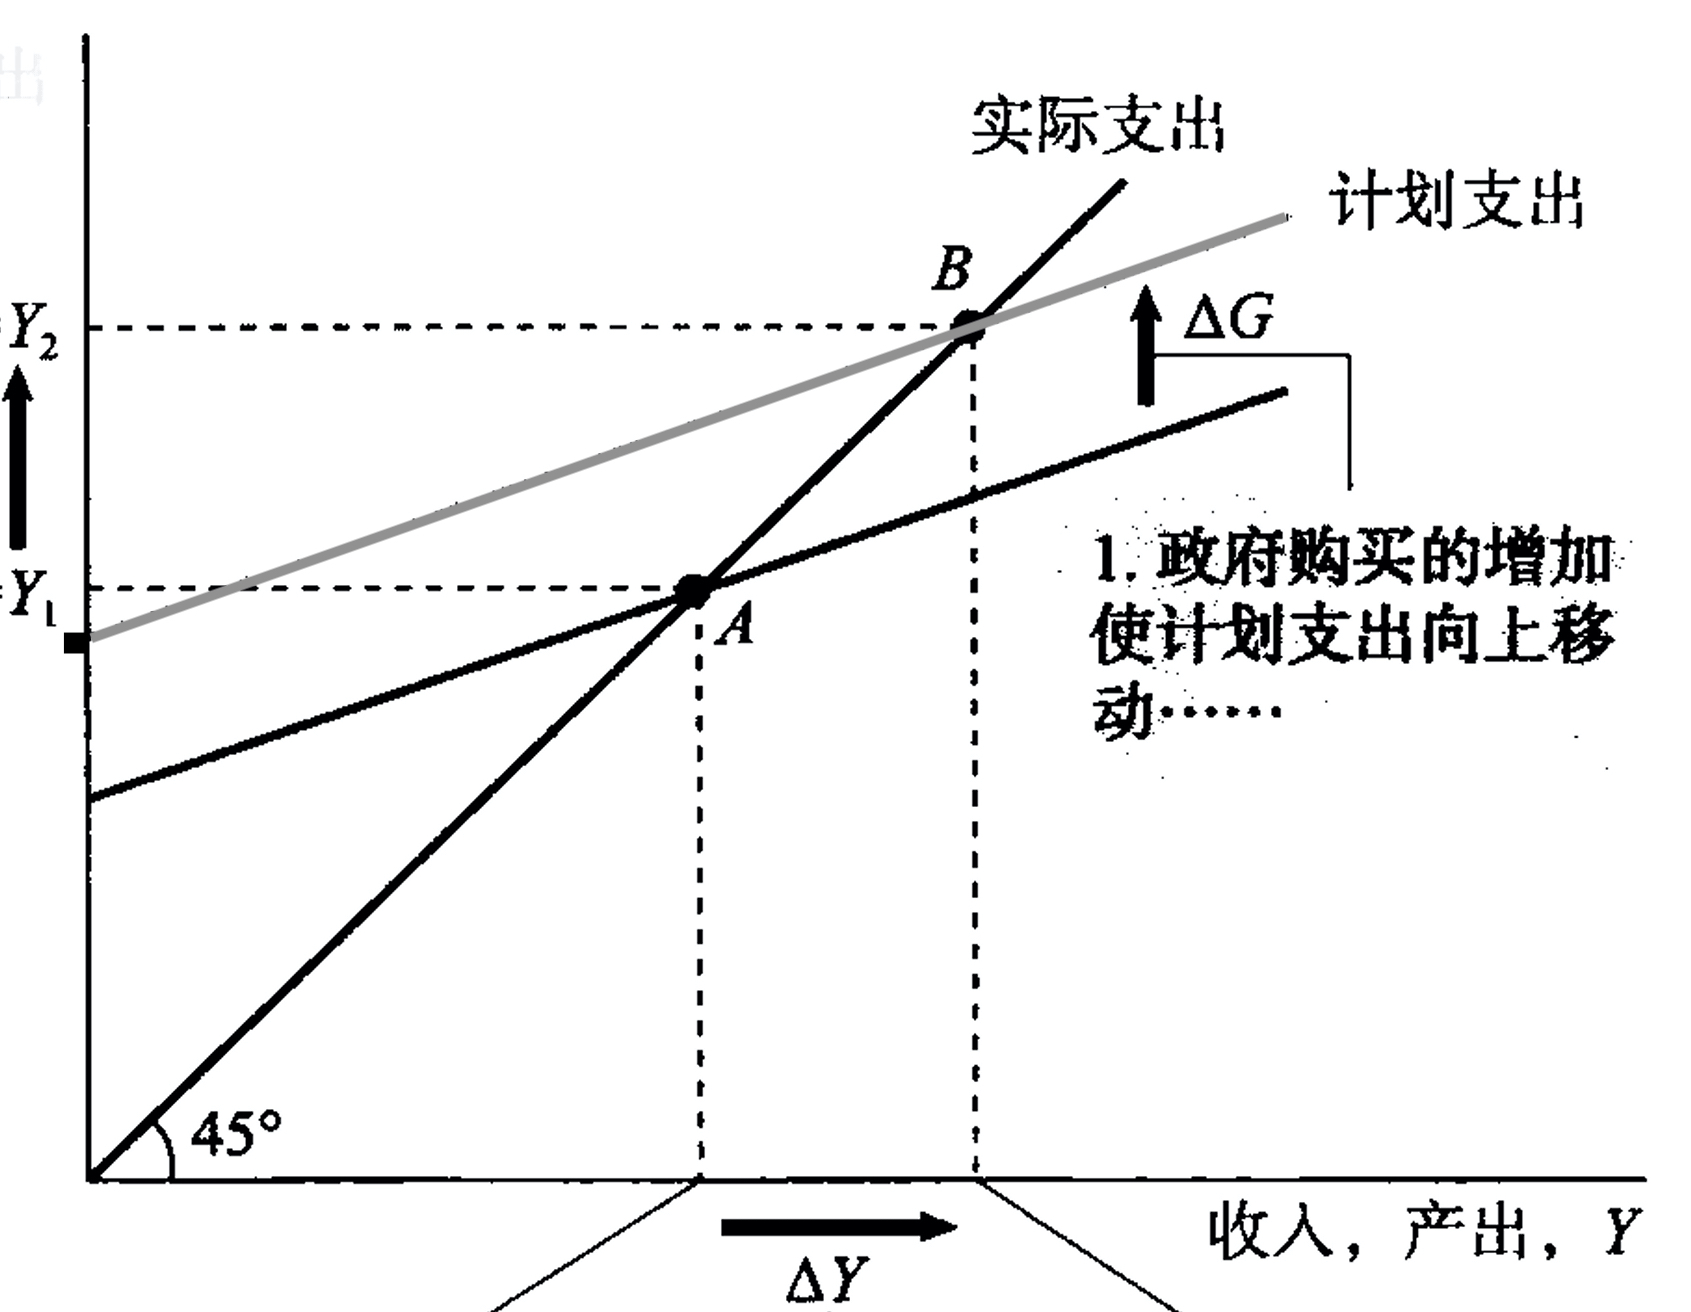
\includegraphics[width=.9\linewidth]{../../fig/ch10-1.jpeg}
%    \caption{政府购买乘数}

\end{minipage}%
\begin{minipage}{.4\textwidth}
  \begin{itemize}
  \item 
    图2:  政府购买乘数
  \item 
    政府购买增加1单位, 即自发性支出增加1单位. 
  \item
    政府购买乘数:$\frac{1}{1-\beta}$, 等于(自发性)支出乘数
  \end{itemize}
\end{minipage}
\end{figure}

\item
  税收乘数: 税收减少 $\Delta T$,  则消费支出上升 $\beta \Delta T$, 
  再乘上(自发性)支出乘数, 可知均衡产出上升 $\frac{\beta}{1- \beta} \Delta T $.
  
  图 3: $T$ 下降 $\Rightarrow$ 计划支出线上移 $\Rightarrow$ 总产出扩张 $\beta/ (1-\beta)$ 倍
\begin{figure}[H]
\centering
\begin{minipage}{.55\textwidth}
  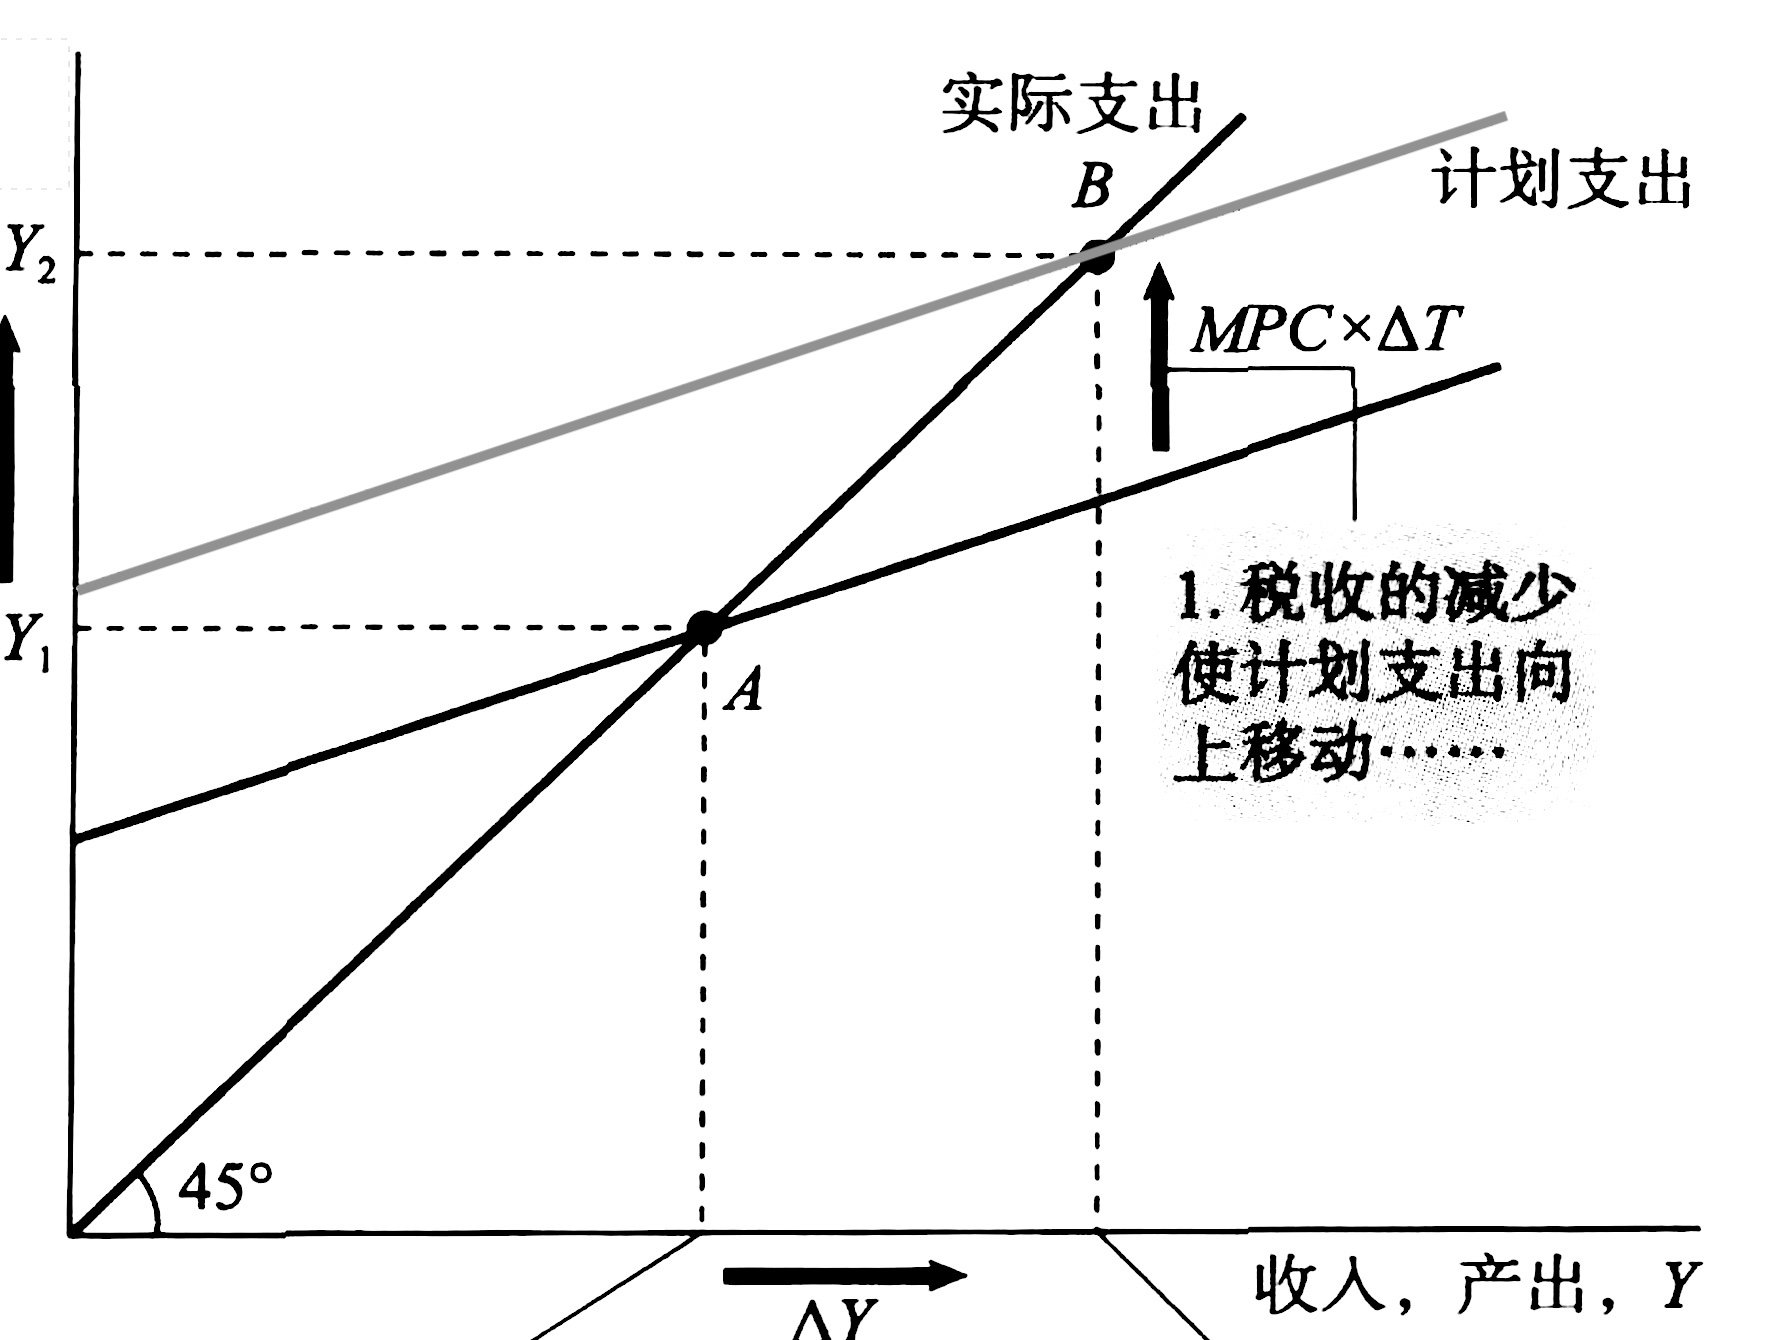
\includegraphics[width=.9\linewidth]{../../fig/ch10-2.jpg}
%    \caption{税收乘数}
\end{minipage}%
\begin{minipage}{.4\textwidth}

  \begin{itemize}
  \item 
    图3: 税收乘数
  \item 
    税收下降1单位, 自发性支出提高 $\beta$ 单位.  ($C$ 提高)
  \item 
    因此, 税收乘数是支出性乘数的 $-\beta$ 倍,  即 $- \frac{\beta}{1- \beta}$.
  \item 注意税收乘数里的负号. \\ 税收下降 $\Rightarrow$ 均衡产出上升 
  \end{itemize}
\end{minipage}
\end{figure}
\item 
  平衡预算乘数: 同时增加等量的税收$T$和政府购买$G$.
  \begin{itemize}
    \item   
    政府购买增加1单位, 使均衡产出上升 $1/ (1-\beta)$;税收增加1单位, 使均衡产出下降 $\beta/ (1-\beta)$.
    两者相减, 总产出增加1单位. 故平衡预算乘数等于1.
    \item
    平衡预算乘数 = 政府购买乘数 + 税收乘数
  \end{itemize}
\end{enumerate}
\end{document}
